\documentclass[a4paper,12pt]{article}

% Pacchetti
\usepackage[utf8]{inputenc}
\usepackage[T1]{fontenc}
\usepackage{lmodern}
\usepackage{graphicx}
\usepackage{amsmath, amssymb}
\usepackage{listings}
\usepackage{xcolor}
\usepackage{geometry}
\geometry{margin=1in}

\usepackage[backend=biber, sorting=nyt, style=enc]{biblatex}
\addbibresource{devoir_spatial.bib}

\usepackage{hyperref}

% Impostazioni per il codice
\lstdefinestyle{mystyle}{
	backgroundcolor=\color{gray!10},   
	commentstyle=\color{green!50!black},
	keywordstyle=\color{blue},
	numberstyle=\tiny\color{gray},
	stringstyle=\color{red},
	basicstyle=\ttfamily\footnotesize,
	breaklines=true,
	captionpos=b,
	keepspaces=true,
	numbers=left,
	numbersep=5pt,
	showspaces=false,
	showstringspaces=false,
	showtabs=false,
	tabsize=4
}

\lstset{style=mystyle}

\setlength{\parindent}{0pt}

\setlength{\skip\footins}{25pt}

% Titolo e Autore
\title{Spatial Analysis Project Report}
\author{Francesco Paolo Savatteri}
\date{\today}

\begin{document}
	
	\maketitle
	
	\vspace{2em}
	
	\begin{abstract}
This report presents a spatial and network analysis approach for evaluating public transport accessibility. Most approaches used in research on the subject use static data, failing to capture real-time mobility conditions.
To address these limitations, this paper proposes a dynamic data-driven methodology using the Google Maps API. By analyzing real-time travel times across different locations in Paris, this paper wants to provide a more accurate representation of urban mobility patterns. However, the approach presented has several limitations that need to be addressed before it can be applied on a large scale.
	\end{abstract}

\pagebreak

\tableofcontents

\newpage

\section{Introduction}
The world's population is becoming increasingly centralized in urban agglomerations. According to World Bank data\footcite{worldbank_data}, today 57\% of the world's population lives in urban areas - in 2000 this figure was 10 points lower, 47\%. This trend is even more pronounced for upper-middle-income countries, where the figure rose from 48\% to 69\% in the same years. A growth of 20 percentage points. \\

In such a context, the mode of transportation of people in cities is an essential element to be studied and analyzed. Public transportation, understood as the set of buses, subways, trains and other non-private means of transportation, has very profound implications in the dynamics of cities. As has been shown by various researchers \footcite{verbavatz2019}, efficient public transportation is the best way to reduce the number of cars in a city and consequently also the level of congestion and CO2 emissions.\\
Other studies focus on how public transportation affects the physical and mental health of people who routinely take public transportation. Researchers have found that taking public transportation equates to a range of 8-33 additional minutes of walking, and this has beneficial effects on those who take it\footcite{rissel2012}. At the same time, however, other studies have shown that commute distances on public transportation are associated with some negative effects such as increased stress\footcite{norgate2020}. \\
Finally, several researches have shown how public transportation also has profound implications in combating social exclusion of marginalized groups\footcite{hine2017}. \\

In light of all this, the objective of this paper is to present a methodology for analyzing public transportation accessibility, using the city of Paris as a case study. “Accessibility” refers to the ability of public transportation to allow people to easily reach their destination. In other words, \emph{how well public transportation works}.

\section{Accessibility measures}

Many ways to measure the accessibility and performance of public transportation have been proposed.\\
A consistent overview has been provided by an article entitled \emph{Public Transport Accessibility: A Literature Review}.\footcite{saif2019}
As the researchers point out, many of the measures of public transportation accessibility focus on specific aspects, such as the reachability of workplaces and the reachability of other types of services (such as schools, hospitals, and the like)\footcite{fransen2015}. While this is a good method, it does not consider all trips that are not related to the use of specific services - for example, visiting a friend or taking a walk in a particular neighborhood.\\
Other approaches use passenger perceptions as measures, through surveys and questionnaires\footcite{lattman2016}. While this method makes it possible to analyze aspects that are difficult to measure otherwise - such as staff courtesy, comfort, and cleanliness of vehicles - it is difficult to apply on a large scale.\\
Finally, other studies have used criteria more specifically related to mobility, through indicators such as mean of numbers of trips and person-miles covered. The main problem with these approaches is that static data, usually the time schedules of the companies providing transportation, are used\footcite{cheng2018}. Depending on the reference context, these data can be far removed from reality and do not take into account factors such as the frequency of breakdowns and contingencies of various kinds.

\section{Methodology}
The objective of our methodology is to measure the ease of mobility within an urban environment from different starting points. In this study, we will focus on Paris as our case study. By analyzing various locations across the city, we aim to assess how accessibility varies depending on the point of origin, providing insights into the spatial dynamics of urban mobility.\\
Unlike the methodologies analyzed so far, we will utilize dynamic data provided by the Google Maps API. This approach allows for a more realistic estimation of travel times between different areas of the city compared to relying on static timetables from transportation companies.

\subsection{Geographic data}
The first step of our methodology involves acquiring and cleaning geographic data. For Paris, we downloaded shapefiles of the city's various arrondissements from the official website of the Mairie de Paris\footcite{paris_arrondissement}. Additionally, we obtained the shapefile containing the city's green areas from the same source\footcite{espaces_verts}. This allowed us to exclude green areas from the original map of the arrondissements. This exclusion is crucial, as considering large parks and green zones would distort the estimation of public transport accessibility. Such areas naturally lack easily accessible public transport options, and including them would lead to an unrealistic assessment of urban mobility.

\subsection{Points coordinates}

Subsequently, we identified 100 points within the map, uniformly distributed using the Poisson Disk Sampling algorithm\footcite{bridson2007}. This algorithm ensures a minimum distance between all points, thereby avoiding the formation of clusters that could occur with a completely random distribution. This uniform distribution is essential for maintaining the spatial consistency necessary for accurate mobility analysis.\\

The map below illustrates the location of 100 points distributed across the city of Paris. The minimum distance between each point is approximately 1,100 meters. Ideally, having more points placed closer together would improve the granularity of the analysis. However, due to computational constraints, we have limited the number of points to 100 in this study.

\begin{figure}[h!]
	\centering
	\includegraphics[width=1\textwidth]{images/coords.png}
	\caption{Location of 100 points in Paris}
	\label{fig:coords_points}
\end{figure}

\subsection{API requests and modelling}

Starting from these points, we calculated the travel times between all pairs of points using the Google Maps API. To avoid excessive costs, the order of the points was not considered: for example, we calculated the travel time from point A to point B and assumed that the travel time from point B to point A would be the same. This approach effectively halved the number of API requests made to Google.\\

At this stage, the data can be conceptualized as a network with multiple nodes, where each node represents a specific point within the city. The network is fully connected, meaning each node is linked to every other node. Each edge connecting a pair of nodes - such as node A and node B - has a temporal attribute corresponding to the travel time calculated by Google Maps for the journey from point A to point B. \\

Mathematically, these data are represented as an adjacency matrix $M$: a 100x100 square matrix in which each element corresponds to the travel time between two nodes. For example, the element $M_{AB}$ represents the travel time from node A to node B.

\subsection{Visualization and analysis}

As an initial application, we created an interactive map\footnote{\url{https://savaij.github.io/map_paris/mappa_interattiva.html}} to visualize the connectivity patterns between nodes as a function of travel time. In other words, based on a selected threshold, the map displays all connections between node pairs with travel times below that threshold. It is important to note that each connection is considered individually concerning the pair of nodes it links. In cases where users wish to identify "paths" (e.g., traveling from node A to node C via node B), the total travel time will exceed the selected threshold even if all pairwise connections are already visible on the map. The image below shows an example of the map with a selected time of 12 minutes.

\begin{figure}[h!]
	\centering
	\includegraphics[width=0.8\textwidth]{images/interactive_map.png}
	\caption{A screenshot of the interactive map}
	\label{fig:interactive_maps}
\end{figure}

Subsequently, we performed analyses by aggregating travel times for each arrondissement. We assigned each point to its corresponding arrondissement and then calculated, for each arrondissement, both the average and maximum travel times for all journeys originating from that arrondissement. For clarity, consider the example of the 15th arrondissement. First, we isolated all points belonging to the 15th arrondissement. Then, we computed the average and the maximum of all travel times for trips that originated from any of these isolated points. The map is accessible online\footnote{\url{https://public.flourish.studio/visualisation/21416572/}}. \\

As can be observed from the images below, it is evident that the more central districts are better connected. This is not surprising. In contrast, it is interesting to note that the 20th arrondissement is particularly poorly connected compared to others. Additionally, the maximum travel times show significant discrepancies from the average in the case of the southern arrondissements. This is because these arrondissements tend to be larger, resulting in greater variability in travel times depending on whether the originating points are more centrally or peripherally located within the arrondissement.

\begin{figure}[h!]
	\centering
	\begin{minipage}{0.48\textwidth}
		\centering
		\includegraphics[width=\linewidth]{images/flourish_map_mean.png} % Prima immagine
		\caption{Mean travel times for arrondissement}
		\label{fig:immagine1}
	\end{minipage}\hfill
	\begin{minipage}{0.48\textwidth}
		\centering
		\includegraphics[width=\linewidth]{images/flourish_map_max.png} % Seconda immagine
		\caption{Max travel times for arrondissemente}
		\label{fig:immagine2}
	\end{minipage}
\end{figure}

For a more in-depth analysis of public transport accessibility in each arrondissement, we constructed an accessibility index. To understand how this index was built, it is necessary to first define a filter function. This function takes as arguments an adjacency matrix $M$  and a time threshold $t$, and returns the number of edges (i.e., elements of the matrix) with a value lower than $t$.

\[
filter(M, t) = n, \quad \text{where } n \in \mathbb{R}
\]

To clarify this concept, let us consider an example. Imagine a network with three nodes: A, B, and C. This network corresponds to a 3x3 adjacency matrix like the one below:

\[
\begin{pmatrix}
	t_{AA} & t_{AB} & t_{AC} \\
	t_{BA} & t_{BB} & t_{BC} \\
	t_{CA} & t_{CB} & t_{CC}
\end{pmatrix}
\]

For the sake of this example, we populate this matrix with arbitrary values as follows. Of course the diagonal elements are not defined because there is no sense in defining a time to go from A to A:

\[
M =
\begin{pmatrix}
	nd & 41 & 17 \\
	35 & nd & 46 \\
	12 & 50 & nd
\end{pmatrix}
\]

Now, we apply the filter function to this matrix using $t=20$ . In this case, $filter(M,20)=2$, meaning that there are two edges in the matrix with values lower than 20. To analyze the behavior of this function over time for the various arrondissements of Paris, we applied this function using 200 values of  ranging from 0 to 80 minutes. Each time, we filtered the travel times based on the arrondissement of departure, allowing for disaggregated statistics for each arrondissement.\\

Additionally, we normalized the results so that all values fall within the range of 0 to 1, ensuring comparability across different arrondissements. For each arrondissement, we have 200 values representing the proportion of trips that take less than time t, as illustrated in the graph below. 

\begin{figure}[h!]
	\centering
	\includegraphics[width=1\textwidth]{images/reached_nodes.png}
	\caption{Share of edges whose duration is less than time t for each arrondissement}
	\label{fig:arr_areas}
\end{figure}

The graph clearly shows that some arrondissements, such as the 1st and 2nd, reach a proportion of 1.0 much faster than others, like the 20th. This indicates that, for example, if only 30 minutes are available, a significantly larger number of destinations within the city can be reached from the 1st and 2nd arrondissements compared to the 20th. \\

Quantitatively, this aspect can be captured by calculating the area under each curve. By comparing the normalized data, we can assess the accessibility conditions of each arrondissement. This measure corresponds to the previously mentioned accessibility index. The closer the value is to 1.0, the higher the accessibility of the neighborhood. This index provides a standardized metric to evaluate spatial disparities in urban mobility and allows for direct comparisons between different areas. \\

\begin{table}[h!]
	\centering
	\begin{tabular}{|c|c|}
		\hline
		\textbf{Arrondissement} & \textbf{Accessibility Index} \\
		\hline
		1  & 0.6670 \\
		2  & 0.6659 \\
		6  & 0.6565 \\
		\hline
		\multicolumn{2}{|c|}{\dots} \\
		\hline
		16 & 0.5673 \\
		19 & 0.5612 \\
		20 & 0.5370 \\
		\hline
	\end{tabular}
	\caption{Value of accessibility index for some arrondissement}
	\label{tab:arrondissement}
\end{table}

Finally, the last stage of the analysis involves an interactive visualization of the average travel times for each point on the map. Depending on the average time, each point is assigned a buffer zone with varying color intensity. More intense colors correspond to higher travel times. Compared to an arrondissement-based aggregation, this visualization better captures the gradual increase in travel times as one moves away from the city center. The map is accessible online\footnote{\url{https://savaij.github.io/map_paris/paris_buffers.html}}.

\begin{figure}[h!]
	\centering
	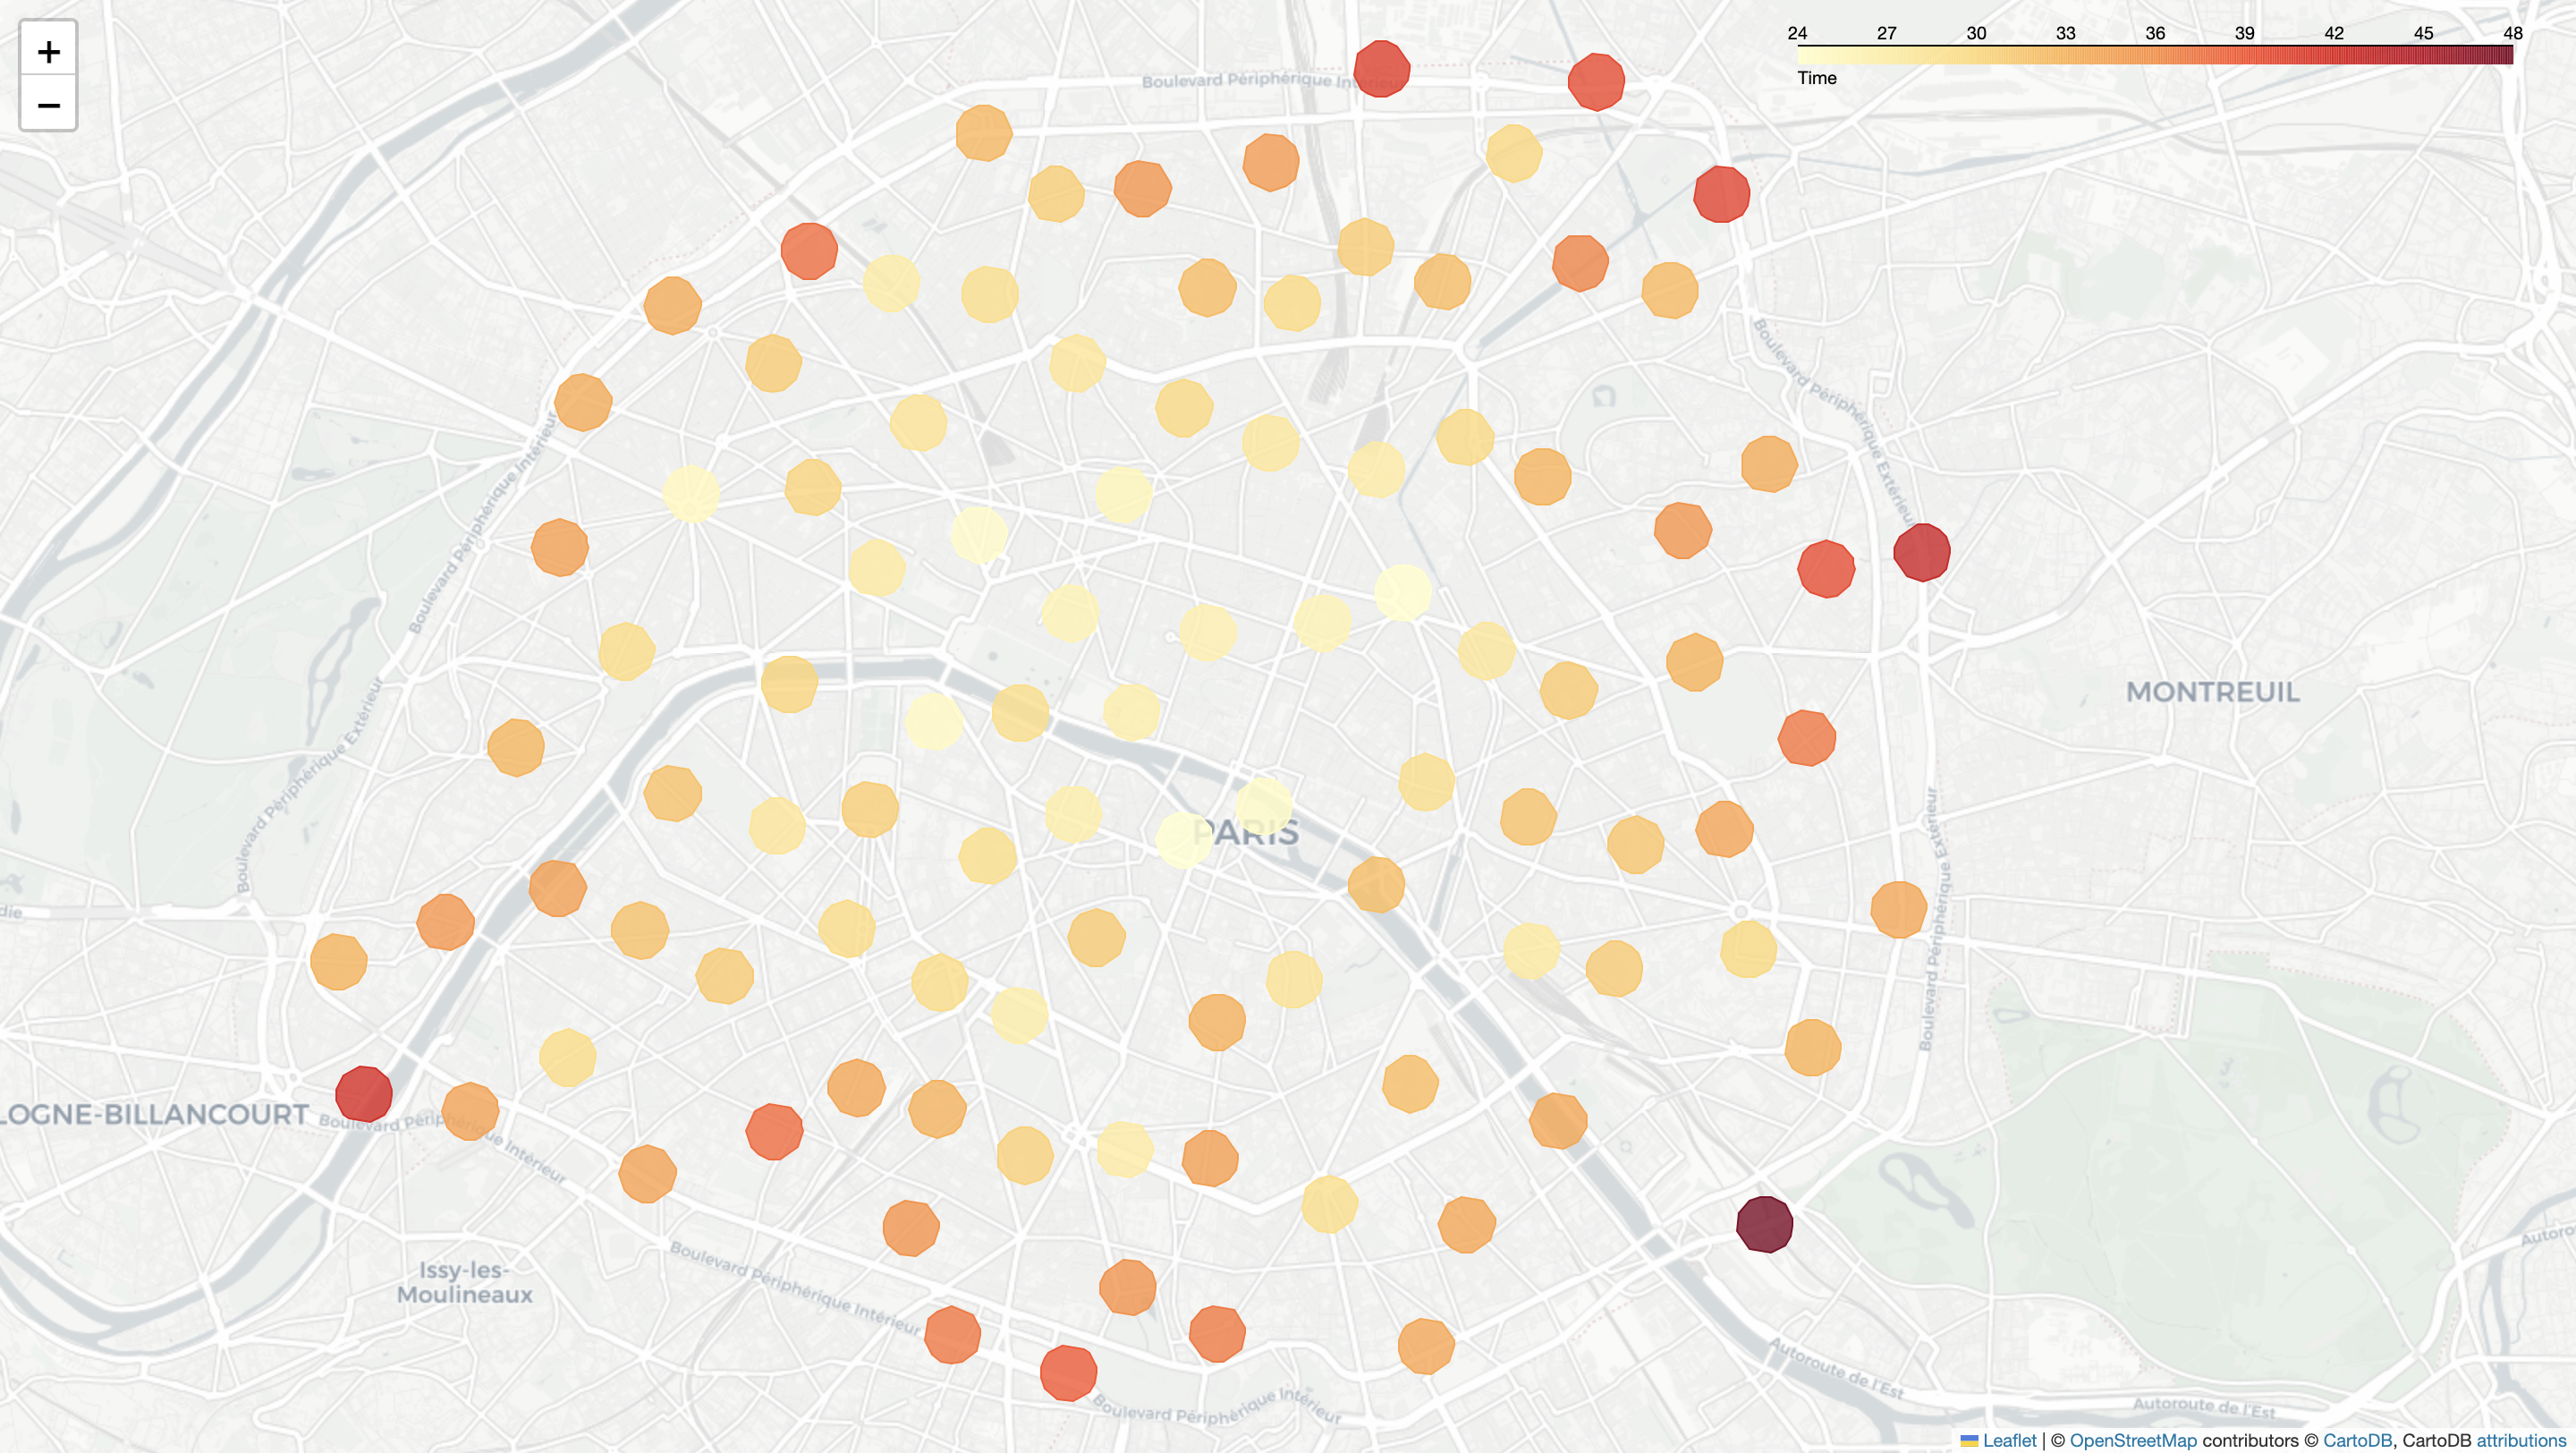
\includegraphics[width=0.8\textwidth]{images/point_by_point.png}
	\caption{A screenshot of the map}
	\label{fig:point_by_point}
\end{figure}

\section{Limitations and future perspectives}
There are several limitations to the approach used in this study. The first limitation concerns the number of points used to create the network nodes. Ideally, the closer and more numerous the points, the more accurate the analysis will be. However, this can significantly increase both economic and computational costs, making the approach impractical. Further research is needed to determine the optimal number of nodes based on the area under study.\\
The second limitation relates to economic costs. Google Maps API is highly precise but comes with considerable expenses. For a sufficiently high number of nodes, costs can easily reach hundreds of euros, making it challenging to apply this methodology on a large scale. \\

Despite these limitations, this approach offers interesting prospects for application. First, it can be used to compare different cities. In particular, the construction of the index, with normalized values, makes such comparisons straightforward. Furthermore, this methodology can be correlated with other sociological aspects, such as the wealth levels of different urban areas, to analyze accessibility disparities across neighborhoods based on additional factors\footnote{All code and data used in this paper can be found here:\url{https://github.com/savaij/paris_transport_accessibility}}.

\newpage

\printbibliography
	

\end{document}